\documentclass[Royal,times,sageh]{sagej}
%DIF LATEXDIFF DIFFERENCE FILE
%DIF DEL main_EPB_v0.tex   Thu May 18 12:24:40 2023
%DIF ADD main_EPB.tex      Fri May 19 10:02:42 2023

\usepackage{moreverb,url,natbib, multirow, tabularx}
\usepackage[colorlinks,bookmarksopen,bookmarksnumbered,citecolor=red,urlcolor=red]{hyperref}



% tightlist command for lists without linebreak
\providecommand{\tightlist}{%
  \setlength{\itemsep}{0pt}\setlength{\parskip}{0pt}}



\usepackage[linesnumbered,lined,boxed,commentsnumbered]{algorithm2e}
\usepackage{booktabs}
\usepackage{longtable}
\usepackage{array}
\usepackage{multirow}
\usepackage{wrapfig}
\usepackage{float}
\usepackage{colortbl}
\usepackage{pdflscape}
\usepackage{tabu}
\usepackage{threeparttable}
\usepackage{threeparttablex}
\usepackage[normalem]{ulem}
\usepackage{makecell}
\usepackage{xcolor}
%DIF PREAMBLE EXTENSION ADDED BY LATEXDIFF
%DIF UNDERLINE PREAMBLE %DIF PREAMBLE
\RequirePackage[normalem]{ulem} %DIF PREAMBLE
\RequirePackage{color}\definecolor{RED}{rgb}{1,0,0}\definecolor{BLUE}{rgb}{0,0,1} %DIF PREAMBLE
\providecommand{\DIFaddtex}[1]{{\protect\color{blue}\uwave{#1}}} %DIF PREAMBLE
\providecommand{\DIFdeltex}[1]{{\protect\color{red}\sout{#1}}}                      %DIF PREAMBLE
%DIF SAFE PREAMBLE %DIF PREAMBLE
\providecommand{\DIFaddbegin}{} %DIF PREAMBLE
\providecommand{\DIFaddend}{} %DIF PREAMBLE
\providecommand{\DIFdelbegin}{} %DIF PREAMBLE
\providecommand{\DIFdelend}{} %DIF PREAMBLE
\providecommand{\DIFmodbegin}{} %DIF PREAMBLE
\providecommand{\DIFmodend}{} %DIF PREAMBLE
%DIF FLOATSAFE PREAMBLE %DIF PREAMBLE
\providecommand{\DIFaddFL}[1]{\DIFadd{#1}} %DIF PREAMBLE
\providecommand{\DIFdelFL}[1]{\DIFdel{#1}} %DIF PREAMBLE
\providecommand{\DIFaddbeginFL}{} %DIF PREAMBLE
\providecommand{\DIFaddendFL}{} %DIF PREAMBLE
\providecommand{\DIFdelbeginFL}{} %DIF PREAMBLE
\providecommand{\DIFdelendFL}{} %DIF PREAMBLE
%DIF HYPERREF PREAMBLE %DIF PREAMBLE
\providecommand{\DIFadd}[1]{\texorpdfstring{\DIFaddtex{#1}}{#1}} %DIF PREAMBLE
\providecommand{\DIFdel}[1]{\texorpdfstring{\DIFdeltex{#1}}{}} %DIF PREAMBLE
%DIF LISTINGS PREAMBLE %DIF PREAMBLE
\RequirePackage{listings} %DIF PREAMBLE
\RequirePackage{color} %DIF PREAMBLE
\lstdefinelanguage{DIFcode}{ %DIF PREAMBLE
%DIF DIFCODE_UNDERLINE %DIF PREAMBLE
  moredelim=[il][\color{red}\sout]{\%DIF\ <\ }, %DIF PREAMBLE
  moredelim=[il][\color{blue}\uwave]{\%DIF\ >\ } %DIF PREAMBLE
} %DIF PREAMBLE
\lstdefinestyle{DIFverbatimstyle}{ %DIF PREAMBLE
	language=DIFcode, %DIF PREAMBLE
	basicstyle=\ttfamily, %DIF PREAMBLE
	columns=fullflexible, %DIF PREAMBLE
	keepspaces=true %DIF PREAMBLE
} %DIF PREAMBLE
\lstnewenvironment{DIFverbatim}{\lstset{style=DIFverbatimstyle}}{} %DIF PREAMBLE
\lstnewenvironment{DIFverbatim*}{\lstset{style=DIFverbatimstyle,showspaces=true}}{} %DIF PREAMBLE
%DIF END PREAMBLE EXTENSION ADDED BY LATEXDIFF

\begin{document}


\setcitestyle{aysep={,}}

\title{A geo-referenced micro-data set of real estate listings for
Spain's three largest cities}

\runninghead{author \emph{et al}.}

\author{\affilnum{}}

\affiliation{}



\begin{abstract}
This article \DIFdelbegin \DIFdel{shares }\DIFdelend \DIFaddbegin \DIFadd{presents }\DIFaddend an open data product with \DIFdelbegin \DIFdel{big }\DIFdelend \DIFaddbegin \DIFadd{large }\DIFaddend geo-referenced
micro-data sets of 2018 real estate listings in Spain. These data were
originally published on the idealista.com real estate website. The
observations were obtained for the three largest cities in Spain: Madrid
(n = 94,815 observations), Barcelona (n = 61,486 observations), and
Valencia (n = 33,622 observations). The data sets include the
coordinates of properties (latitude and longitude), asking prices of
each listed dwelling, and several variables of indoor characteristics.
The listings were enriched with official information from the Spanish
cadastre (e.g., building material quality) plus other relevant
geographical features, such as distance to urban points of interest.
Along with the real estate listings, the data product also includes
neighborhood boundaries for each city. The data product is offered as a
fully documented \DIFdelbegin \DIFdel{R }\DIFdelend \DIFaddbegin \texttt{\DIFadd{R}} \DIFaddend package and is available for scientific and
educational purposes, particularly for geo-spatial studies
\end{abstract}

\DIFdelbegin %DIFDELCMD < \keywords{Housing market; idealista.com; geo-referenced data;
%DIFDELCMD < point-level data; open data; Spain}
%DIFDELCMD < %%%
\DIFdelend \DIFaddbegin \keywords{Housing prices; hedonic price analysis; idealista.com;
geo-referenced data; point-level data; open data; Spain}
\DIFaddend 

\maketitle

\hypertarget{introduction}{%
\section{Introduction}\label{introduction}}

Interest in the characteristics of the housing market and housing prices
has been a growing area of research in recent decades, generating a vast
amount of theoretical and empirical literature. Including the spatial
component to analyze the real estate market and incorporating geographic
variables has significantly improved the understanding of this market\DIFdelbegin \DIFdel{.
But to really understand the characteristics of the housing market}\DIFdelend \DIFaddbegin \DIFadd{:
to this end}\DIFaddend , it is essential to have information/data at the point
level. Therefore, it is becoming common for spatial analysis of urban
environments to be \DIFdelbegin \DIFdel{developed with geo- referenced }\DIFdelend \DIFaddbegin \DIFadd{use }\DIFaddend micro-data\DIFdelbegin \DIFdel{sets \mbox{%DIFAUXCMD
\citep{lopez2015}}\hspace{0pt}%DIFAUXCMD
. However, the availability of this type of open data at the point level
is limited, and not many data sets contain latitude/longitude
coordinates for each dwelling. }\DIFdelend \DIFaddbegin \DIFadd{, geo-referenced as points
\mbox{%DIFAUXCMD
\citep{lopez2015}}\hspace{0pt}%DIFAUXCMD
. }\DIFaddend In some cases, researchers have had to resort to
\DIFdelbegin \DIFdel{web scraping }\DIFdelend \DIFaddbegin \DIFadd{webscraping }\DIFaddend processes to obtain \DIFdelbegin \DIFdel{the large volumes of
information that permit robust analyses
\mbox{%DIFAUXCMD
\citep{gupta2022take, arbia2020spatial, Li2019, lopez2015}}\hspace{0pt}%DIFAUXCMD
. These web
scraping processes can include missing data , }\DIFdelend \DIFaddbegin \DIFadd{data for research
\mbox{%DIFAUXCMD
\citep[e.g.,][]{Li2019, lopez2015}}\hspace{0pt}%DIFAUXCMD
. Alas, webscraping is a chancy
process prone to }\DIFaddend download errors, \DIFdelbegin \DIFdel{duplicate
}\DIFdelend \DIFaddbegin \DIFadd{missing data, duplicated }\DIFaddend records, etc.
Furthermore, \DIFdelbegin \DIFdel{the authors of this research do not generally
share the data sets. }%DIFDELCMD < 

%DIFDELCMD < %%%
\DIFdel{We are also witnessing }\DIFdelend \DIFaddbegin \DIFadd{researchers do not always share their webscrapped datasets,
which limits reproducibility of their research. As we witness }\DIFaddend a growing
interest in \DIFdelbegin \DIFdel{open data in geography and }\DIFdelend \DIFaddbegin \DIFadd{openness and reproducibility in geographical data science
\mbox{%DIFAUXCMD
\citep{arribasl2021editorial, paez2021open, brunsdon2021opening}}\hspace{0pt}%DIFAUXCMD
, it
becomes increasingly urgent to have open }\DIFaddend data \DIFdelbegin \DIFdel{science \mbox{%DIFAUXCMD
\citep{arribasl2021editorial, arribas2021} }\hspace{0pt}%DIFAUXCMD
using
reproducible or replicable research
\mbox{%DIFAUXCMD
\citep{paez2021open, brunsdon2021opening}}\hspace{0pt}%DIFAUXCMD
. But to work openly in
science, it
is necessary to have free software and open data . While
great efforts have been made to make free software availableto
researchers (e.g., R or Python), data regarding }\DIFdelend \DIFaddbegin \DIFadd{products to support
research \mbox{%DIFAUXCMD
\citep{arribas2021}}\hspace{0pt}%DIFAUXCMD
.
}

\DIFadd{Some researchers have already responded to this need for publicly
available, geo-referenced datasets to support open, reproducible
research. A few such datasets are now available to support the analysis
of }\DIFaddend real estate markets\DIFdelbegin \DIFdel{tend
to be treated as confidential, and there are still few open micro-data
sets of housing markets available \mbox{%DIFAUXCMD
\citep{Song2021}}\hspace{0pt}%DIFAUXCMD
. }\DIFdelend \DIFaddbegin \DIFadd{, but they are sometimes geo-referenced at the
level of large geographical zones, such as \mbox{%DIFAUXCMD
\citet{fuerst2020real}}\hspace{0pt}%DIFAUXCMD
, an
open dataset that includes \(n=4,201\) property prices geocoded to the
level of nine regions in England and Wales. Other datasets are geo-coded
as points, including \mbox{%DIFAUXCMD
\citet{bonifaci2015real}}\hspace{0pt}%DIFAUXCMD
, which includes
\(n=1,042\) observations for Padua, in Italy;
\mbox{%DIFAUXCMD
\citet{delgiudice2018housing}}\hspace{0pt}%DIFAUXCMD
, who share a dataset with \(n=576\)
observations relating to rental prices in Naples, Italy; and
\mbox{%DIFAUXCMD
\citet{solano2019dataset} }\hspace{0pt}%DIFAUXCMD
present a dataset with \(n=1,623\) daily
rental prices in Seville, Spain.
}\DIFaddend 

To contribute to the growing inventory of international micro-data sets
of real estate markets, this paper introduces an open \DIFdelbegin \DIFdel{micro-data set of
}\DIFdelend \DIFaddbegin \DIFadd{data product with
}\DIFaddend geo-referenced dwelling listings\DIFaddbegin \DIFadd{, called \{idealista18\}}\DIFaddend . The data have
been provided by the Idealista
company\footnote{Idealista is the major real estate listing website in Spain, and present in other southern european countries as Italy and Portugal}
and contain information about 189,923 dwellings located in Spain's three
largest cities. To date, this data product is \DIFdelbegin \DIFdel{the biggest }\DIFdelend \DIFaddbegin \DIFadd{one of the largest }\DIFaddend open
geo-referenced micro-data set of the housing market in \DIFdelbegin \DIFdel{Spain. Moreover, the data }\DIFdelend \DIFaddbegin \DIFadd{the world. The
most similar in terms of geographical disaggregation and sample size is
the dataset of \mbox{%DIFAUXCMD
\citet{song2021hedonic} }\hspace{0pt}%DIFAUXCMD
which includes transactions for
four cities in South Korea, namely Busan (\(n=61,152\)), Daegu
(\(n=32,363\)), Daejeon (\(n=21,114\)), and Gwangju (\(n=25,984\)).
\{idealista18\} is certainly the largest open data product of its kind
in Spain.
}

\DIFadd{The data }\DIFaddend set has been supplied directly by Idealista, and therefore is
clean and free \DIFdelbegin \DIFdel{of }\DIFdelend \DIFaddbegin \DIFadd{from }\DIFaddend download errors. However, \DIFdelbegin \DIFdel{in order to be able to share
publicly the data
we have slightly modified some variables by applying some random noise which }\DIFdelend \DIFaddbegin \DIFadd{to comply with data
legislation, we have masked the prices by applying a small amount of
random noise that }\DIFaddend will not bias the main results derived from its usage.

This micro-data set \DIFdelbegin \DIFdel{is expected to be used as a benchmark dataset to test empirical }\DIFdelend \DIFaddbegin \DIFadd{can be used to benchmark new }\DIFaddend methods in a
reproducible fashion \DIFaddbegin \DIFadd{\mbox{%DIFAUXCMD
\citep[e.g.,][]{rey2023using}}\hspace{0pt}%DIFAUXCMD
}\DIFaddend . Applied and
theoretical researchers on real estate mass appraisal and valuation
methods might use this dataset to canonically compare the performance of
their proposed comparable and hedonic models, among others. The data can
also be used to study the segmentation of housing submarkets and related
topics such as the impact of suburban areas on house prices. The
listings have been enriched with official information from the Spanish
cadastre along with other relevant geographical features, such as
distance to urban points of interest. In any case, the data might be
easily extended by spatially joining other datasets that contain
information at administrative, census tract, or postal code levels.

The data set is distributed as an \DIFdelbegin \DIFdel{R package , name \{idealista18\}, which
}\DIFdelend \DIFaddbegin \texttt{\DIFadd{R}} \DIFadd{package and it }\DIFaddend can be
accessed from a public Github
repository\footnote{\DIFdelbegin \DIFdel{The direct URL to the GitHub repository is }\DIFdelend \url{https://github.com/paezha/idealista18}}. The
\DIFdelbegin \DIFdel{database idealista18 }\DIFdelend \DIFaddbegin \DIFadd{open data product }\DIFaddend is made available under the
\href{http://opendatacommons.org/licenses/odbl/1.0/}{Open Database License}.
For transparency, we also share the \DIFdelbegin \DIFdel{randomisation }\DIFdelend \DIFaddbegin \DIFadd{masking }\DIFaddend process applied to the
original data in the aforementioned Github repository.

\hypertarget{data-description}{%
\section{Data description}\label{data-description}}

The open data product \{idealista18\} is an \DIFdelbegin \DIFdel{R }\DIFdelend \DIFaddbegin \texttt{\DIFadd{R}} \DIFaddend package composed
of \DIFdelbegin \DIFdel{nine
}\DIFdelend \DIFaddbegin \DIFadd{ten }\DIFaddend objects, three objects for each of the three main Spanish cities:
Barcelona, Madrid, and Valencia. For each city, dwelling listings,
neighborhood polygons, and a set of points of interest have been
included in the \DIFdelbegin \DIFdel{R package. }\DIFdelend \DIFaddbegin \DIFadd{package. There is in addition a data object with the
number of dwellings by district (a collection of neighborhoods),
according to the Spanish cadastre.
}

\DIFadd{The data provider (idealista.com) is a leading real estate portal in
Spain, on par with its nearest competitor Fotocasa. Smaller listing
portals include Habitaclia and Milanuncios, the latter focusing almost
exclusively on individual (i.e., non-professional) advertisers. In
September 2021, according to data from Similarweb (a site specialized in
sites' traffic volume comparison), there were a total of 103 million
page views on real estate portals in Spain. Of this, 94\% of traffic was
concentrated on four portals, of which idealista was the most important,
followed by Fotocasa, Habitaclia, and Pisos.com. Traffic is also highly
concentrated, and idealista.com was the the leader by far with 58.6
monthly million visits (57\% of the total traffic) compared to its
closest competitor with 19.9 million visits (19.3 \% of total traffic).
}

\DIFadd{As a result of its share of advertisments, idealista.com covers fairly
well all segments of the Spanish market, including both individual and
professional advertisers. This dataset includes information about
listing prices, and therefore represents the market situation from the
perspective of asking prices. This is a necessary compromise in the
present case, since actual sale prices are not publicly available, and
the information can only be accessed by paying high fees to Colegio de
Registradores. However listing prices reflect quite well the
(transaction) reality of real estate markets, and correlations between
idealista listings and transaction prices can be established see
}\href{https://papers.ssrn.com/sol3/papers.cfm?abstract_id=3400031}{\DIFadd{Banco
de España}}\DIFadd{. Official transactions and asking prices can be taken as
complementary and are of great interest when studying asking-transaction
price gaps or the relation between listing site demand variables (i.e.,
ad contacts or ad views) and price gaps.
}

\DIFadd{To provide some context about the coverage of the \{idealista18\}
dataset Table \ref{tab:transactions} shows the number of listings with
respect to the total residential stock in each city in 2018. As seen in
the table, the number of listings ranges between 6.1\% of the total
number of properties (in Madrid) and 8.1\% (in Valencia). Information
from Instituto Nacional de Estadistica}\footnote{\url{https://www.ine.es/jaxiT3/Tabla.htm?t=6150&L=1}}
\DIFadd{shows that the number of listings in the \{idealista18\} package
correspond to 81.3\% of recorded real estate transactions in Barcelona,
80.8\% in Madrid, and 91.1\% in Valencia.
}

\begin{table}[!ht]
\centering
\caption{\DIFaddFL{Total properties and transactionst three Spanish cities. Year 2018}} 
\label{tab:transactions} 
\begin{tabular}{lccccc}
\DIFaddFL{City }& \DIFaddFL{Total properties (TP) }& \DIFaddFL{Total transactions (TT) }& \DIFaddFL{Listings (L) }& \DIFaddFL{L/TP }& \DIFaddFL{TT/L }\\
\hline
\DIFaddFL{Barcelona }&  \DIFaddFL{789,740  }&  \DIFaddFL{56,012  }&  \DIFaddFL{61,329  }& \DIFaddFL{7.8\% }& \DIFaddFL{81.3\%  }\\ 
\DIFaddFL{Madrid }&  \DIFaddFL{1,545,397  }&  \DIFaddFL{76,603  }&  \DIFaddFL{94,802  }& \DIFaddFL{6.1\%  }& \DIFaddFL{80.8\% }\\ 
\DIFaddFL{Valencia }&  \DIFaddFL{416,004  }&  \DIFaddFL{30,615  }&  \DIFaddFL{33,593  }& \DIFaddFL{8.1\% }& \DIFaddFL{91.1\% }\\ 
\hline
\DIFaddFL{Total }&  \DIFaddFL{2,751,141  }&  \DIFaddFL{163,230  }&  \DIFaddFL{189,724  }& \DIFaddFL{6.9\% }& \DIFaddFL{86.0\% }\\ 
\hline
\multicolumn{6}{l}{{\footnotesize \textbf{Sources}}}\\
\multicolumn{6}{l}{{\footnotesize Total properties (P): Ministerio Español de Hacienda y Función Pública}}\\
\multicolumn{6}{l}{{\footnotesize Total transactions (T): Instituto Nacional de Estadística}}\\
\end{tabular}
\end{table}

\DIFaddend The following subsections describe \DIFdelbegin \DIFdel{each
object}\DIFdelend \DIFaddbegin \DIFadd{the data objects}\DIFaddend . A full description
of the data is \DIFaddbegin \DIFadd{also }\DIFaddend available in the help section of the package. We
have \DIFdelbegin \DIFdel{strived }\DIFdelend \DIFaddbegin \DIFadd{tried }\DIFaddend to the best of our ability to comply with FAIR principles
regarding research data \citep{Wilkinson2016fair}: upon publication, the
dataset has a persistent digital object identifier; publication as a
data article makes the data findable; the data and metadata are packaged
together and protocols for help files in the \DIFdelbegin \DIFdel{R }\DIFdelend \DIFaddbegin \texttt{\DIFadd{R}} \DIFaddend ecosystem mean
that documentation is easily searchable; distribution as an \DIFdelbegin \DIFdel{R }\DIFdelend \DIFaddbegin \texttt{\DIFadd{R}}
\DIFaddend package means that only open software is needed to access the data; and
a public repository documents all data processes followed to generate
the distributed open data product.

\hypertarget{dwelling-listings}{%
\subsection{Dwelling listings}\label{dwelling-listings}}

The \DIFdelbegin \DIFdel{dwelling listing of }\DIFdelend \DIFaddbegin \DIFadd{listing for }\DIFaddend each city includes a set of characteristics for each
dwelling published on the idealista real estate website\DIFdelbegin \DIFdel{as an ad. The dwelling listing
has been }\DIFdelend \DIFaddbegin \DIFadd{. The listing
}\DIFaddend included in the \DIFdelbegin \DIFdel{`}\DIFdelend \DIFaddbegin \DIFadd{\{}\DIFaddend idealista18\DIFdelbegin \DIFdel{' package as
an sfobject \mbox{%DIFAUXCMD
\citep{Pebesma} }\hspace{0pt}%DIFAUXCMD
}\DIFdelend \DIFaddbegin \DIFadd{\} package are simple features (sf) objects
\mbox{%DIFAUXCMD
\citep{Pebesma} }\hspace{0pt}%DIFAUXCMD
with point geometry in latitude and longitude}\DIFaddend . The name
of \DIFdelbegin \DIFdel{the sf object containing the dwelling listing includes }\DIFdelend \DIFaddbegin \DIFadd{each sf object with the list of dwellings is }\DIFaddend the name of the city
\DIFdelbegin \DIFdel{, }\DIFdelend followed by '\_Sale' (e.g., \DIFdelbegin \DIFdel{Madrid\_Sale)and }\DIFdelend \DIFaddbegin \texttt{\DIFadd{Madrid\_Sale}}\DIFadd{). Each data object
}\DIFaddend includes a total of 42 variables \DIFdelbegin \DIFdel{. Each sf
object includes }\DIFdelend \DIFaddbegin \DIFadd{and }\DIFaddend the complete set of listings
corresponding to the four quarters of \DIFdelbegin \DIFdel{the year 2018. }\DIFdelend \DIFaddbegin \DIFadd{2018 (Q1 through Q4). }\DIFaddend Table
\ref{tab:number-ads} shows the number of dwelling listing ads included
in the data set for each city and quarter. The record counts for each
city are: 94,815 listings for Madrid, 61,486 for Barcelona, and 33,622
for Valencia. Note that the same dwelling may be found in more than one
period when a property listed for sale in one quarter was sold in a
subsequent quarter. The variable ASSETID, included in the sf objects, is
the unique identifier of the dwelling.

\begin{table}[ht]
\centering
\begin{tabular}{>{\raggedright\arraybackslash}p{4em}>{\raggedleft\arraybackslash}p{3em}cccc}
  \hline
City$\backslash$Quarter & First & Second  & \DIFdelbeginFL \DIFdelFL{Thirdr }\DIFdelendFL \DIFaddbeginFL \DIFaddFL{Third }\DIFaddendFL & Fourth & Total ads \\ 
  \hline
Barcelona & 17826 & 7951 & 12375 & 23334 & 61486 \\ 
  Madrid & 21920 & 12652 & 15973 & 44270 & 94815 \\ 
  Valencia & 9305 & 4655 & 5644 & 14018 & 33622 \\ 
   \hline
\end{tabular}
\caption{Number of dwelling  listing ads for each city and quarter. \label{tab:number-ads}} 
\end{table}

Each record of the dwelling listing contains a set of indoor
characteristics supplied by the advertisers on the Idealista website
(e.g., price, surface area, number of bedrooms, basic features, etc.),
including \DIFdelbegin \DIFdel{the exact }\DIFdelend \DIFaddbegin \DIFadd{an approximated }\DIFaddend location of the dwelling (\DIFdelbegin \DIFdel{see }\DIFdelend \DIFaddbegin \DIFadd{the exact location
has been masked, as described in }\DIFaddend Section
\protect\DIFdelbegin %DIFDELCMD < \hyperlink{anonymizing}{Anonymizing the data set}%%%
\DIFdelend \DIFaddbegin \hyperlink{anonymizing}{Masking the prices}\DIFaddend ). Table
\ref{tab:variables} lists the main indoor variables with a short
description and the mean value of each variable. The dwelling listings
were enriched with a number of additional attributes from the Spanish
cadastre \citep{Catastro}. The cadastral information is described in
Table \ref{tab:variables}, with the prefix CAD in the variable name. The
cadastral features were assigned by applying the features of the nearest
parcel to the coordinates. The year the dwelling was built
(CONSTRUCTIONYEAR) given by the advertiser was revised since the year of
construction is entered on the website by users, and it is therefore
subject to errors and incomplete data (40\% missing data). To resolve
this issue, an alternative variable (CADCONSTRUCTIONYEAR) was included,
assigning the cadastral construction year from the nearest cadastral
parcel whenever the value was outstanding (date was after publication
date or year of construction was before 1500) or when the value supplied
by the advertiser was missing.

Additionally, the distance of each dwelling to \DIFdelbegin \DIFdel{three urban }\DIFdelend \DIFaddbegin \DIFadd{several }\DIFaddend points of
interest was included in the sf object: distance to the city center,
distance to the closest metro station, and distance to a major street
(La Diagonal for Barcelona, La Castellana for Madrid, and Blasco Ibañez
for Valencia). The last rows of Table \ref{tab:variables} show the mean
values of these variables.

\begin{table}[ht]
\centering
\fontsize{8}{10}\selectfont
\begin{tabular}{>{\raggedright\arraybackslash}p{13em}>{\raggedright\arraybackslash}p{14em}ccc}
  \hline
Variable & Sort Description & Barcelona & Madrid & Valencia \\ 
  \hline
PRICE & Asking price & 395770.58 & 396110.11 & 199678.31 \\ 
  UNITPRICE & Asking price per m\verb|^|2 (euros) & 4044.86 & 3661.05 & 1714.54 \\ 
  CONSTRUCTEDAREA & Surface (m\verb|^|2) & 95.46 & 101.40 & 108.95 \\ 
  ROOMNUMBER & Number of bedrooms & 2.86 & 2.58 & 3.07 \\ 
  BATHNUMBER & Number of bathrooms & 1.52 & 1.59 & 1.59 \\ 
  CONSTRUCTIONYEAR & Construction year (advertiser) & 1952.58 & 1964.69 & 1969.43 \\ 
  CADCONSTRUCTIONYEAR & Construction year (cadastre) & 1952.19 & 1965.70 & 1970.55 \\ 
  CADMAXBUILDINGFLOOR & Max build floor & 6.85 & 6.38 & 7.04 \\ 
  CADDWELLINGCOUNT & Dwelling count in the building & 28.56 & 39.19 & 36.83 \\ 
  CADASTRALQUALITYID & Cadastral quality. 0 Best-10 Worst & 4.31 & 4.85 & 5.34 \\ 
  DISTANCE\_TO\_CITY\_CENTER & Distance to city center & 2.80 & 4.49 & 2.09 \\ 
  DISTANCE\_TO\_METRO & Distance to subway station & 0.27 & 0.48 & 0.64 \\ 
  DISTANCE\_TO\_(MAINSTREET) & Distance to major street & 1.77 & 2.68 & 2.07 \\ 
   \hline
\end{tabular}
\caption{List, sort description, and mean of the main quantitative variables included in the dwelling listing for the three Spanish cities. See the help section in the \DIFdelbeginFL \textbf{\DIFdelFL{idealista18}} %DIFAUXCMD
\DIFdelFL{R }\DIFdelendFL \DIFaddbeginFL \DIFaddFL{\{idealista18\} }\DIFaddendFL package for details and formal definitions. Some variables have been excluded from this table to save space. Check the full list in the \DIFdelbeginFL \textbf{\DIFdelFL{idealista18}} %DIFAUXCMD
\DIFdelendFL package.\label{tab:variables}} 
\end{table}

In addition to the variables listed in Table \ref{tab:variables}, the sf
object includes a set of dummy variables with information about the
basic characteristics of the dwelling. Table \ref{tab:Dummy-variables}
shows the more relevant variables included in the sf object.

\begin{table}[ht]
\centering
\fontsize{8}{10}\selectfont
\begin{tabular}{>{\raggedright\arraybackslash}p{12em}>{\raggedright\arraybackslash}p{14em}ccc}
  \hline
Variable & Sort Description & Barcelona & Madrid & Valencia \\ 
  \hline
HASTERRACE & =1 if has terrace & 0.33 & 0.36 & 0.25 \\ 
  HASLIFT & =1 if has lift & 0.74 & 0.70 & 0.79 \\ 
  HASAIRCONDITIONING & =1 if has air conditioning & 0.47 & 0.45 & 0.47 \\ 
  HASPARKINGSPACE & =1 if has parking & 0.08 & 0.23 & 0.17 \\ 
  HASNORTHORIENTATION & =1 if has north orientation & 0.13 & 0.11 & 0.13 \\ 
  HASSOUTHORIENTATION & =1 if has south orientation & 0.31 & 0.24 & 0.19 \\ 
  HASEASTORIENTATION & =1 if has east orientation & 0.24 & 0.20 & 0.25 \\ 
  HASWESTORIENTATION & =1 if has west orientation & 0.16 & 0.15 & 0.15 \\ 
  HASBOXROOM & =1 if has boxroom & 0.12 & 0.26 & 0.13 \\ 
  HASWARDROBE & =1 if has wardrobe & 0.30 & 0.57 & 0.53 \\ 
  HASSWIMMINGPOOL & =1 if has swimmingpool & 0.03 & 0.15 & 0.07 \\ 
  HASDOORMAN & =1 if has doorman & 0.08 & 0.25 & 0.05 \\ 
  HASGARDEN & =1 if has garden & 0.04 & 0.18 & 0.06 \\ 
  ISDUPLEX & =1 if is duplex & 0.03 & 0.03 & 0.02 \\ 
  ISSTUDIO & =1 if is studio & 0.02 & 0.03 & 0.01 \\ 
  ISINTOPFLOOR & =1 is on the top floor & 0.02 & 0.02 & 0.01 \\ 
  BUILTTYPEID\_1 & =1 if is new contruction & 0.01 & 0.03 & 0.03 \\ 
  BUILTTYPEID\_2 & =1 is second hand to be restored & 0.17 & 0.19 & 0.13 \\ 
  BUILTTYPEID\_3 & =1 is second hand in good condition & 0.82 & 0.78 & 0.83 \\ 
   \hline
\end{tabular}
\caption{List of dummy variables, sort description, and ratios of dwellings with the specific characteristics. See the help section in the \textbf{idealista18} R package for details and formal definitions. Some dummy variables have been excluded from this table to save space\label{tab:Dummy-variables}} 
\end{table}

\hypertarget{neighboorhood-polygons}{%
\subsection{Neighboorhood polygons}\label{neighboorhood-polygons}}

The second \DIFdelbegin \DIFdel{block of data included in the `}\DIFdelend \DIFaddbegin \DIFadd{data object included in \{}\DIFaddend idealista18\DIFdelbegin \DIFdel{' R package is the spatial features of }\DIFdelend \DIFaddbegin \DIFadd{\} is the neighborhoods
in }\DIFaddend the three cities \DIFdelbegin \DIFdel{divided into neighborhoods}\DIFdelend \DIFaddbegin \DIFadd{as polygons}\DIFaddend . There is an sf object for each city
with the name of the city and the suffix '\_Polygons'. \DIFaddbegin \DIFadd{The left column
of }\DIFaddend Figure \ref{fig:all-polygons} shows the quantile maps of the number
of dwellings in the listing for the different neighborhoods in the three
cities. The neighborhoods are based on the official boundaries but
slightly changed by
Idealista\footnote{There are two criteria used to make this division. If an area is small enough and similar enough to another, the two areas are merged, and, if the official area is not homogeneous, it is divided into a series of new polygons.}.
In practical terms, we can assume they are the same since the website
combines areas when there are few ads for that area. In the case of
Madrid, they combined four areas into two.

\DIFdelbegin %DIFDELCMD < \begin{figure}
%DIFDELCMD < \centering
%DIFDELCMD < 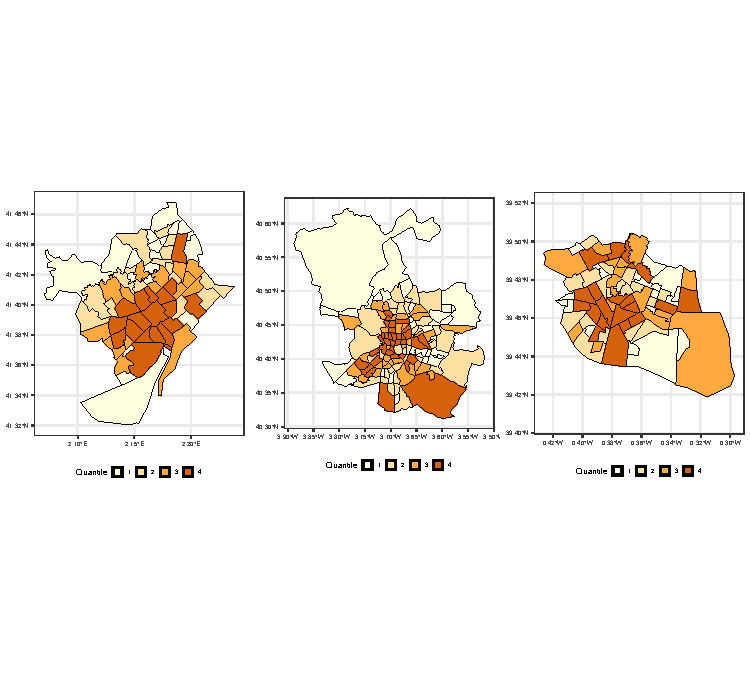
\includegraphics{main_EPB_v0_files/figure-latex/unnamed-chunk-1-1.pdf}
%DIFDELCMD < %%%
%DIFDELCMD < \caption{%
{%DIFAUXCMD
%DIFDELCMD < \label{fig:all-polygons}%%%
\DIFdelFL{Quantile maps of the number of
dwellings in each neighborhood. Boundary for Barcelona (Left), Madrid
(Center), and Valencia (Right).}}
%DIFAUXCMD
%DIFDELCMD < \end{figure}
%DIFDELCMD < 

%DIFDELCMD < %%%
\DIFdelend There are a total of 69 neighborhoods in Barcelona, 135 in Madrid, and
73 in Valencia. The sf object includes a unique identifier (LOCATIONID)
and the neighborhood name (LOCATIONNAME).

\DIFaddbegin \DIFadd{The total number of dwellings is available from the Spanish cadastre
aggregated by district (districts are groups of neighborhoods). The
right column in Figure \ref{fig:all-polygons} shows the percentage of
listed dwellings relative to the total number of dwelling by district in
each of the three cities. This gives a sense of how active residential
real estate markets were in different parts of each city in 2018.
}

\begin{figure}
\centering
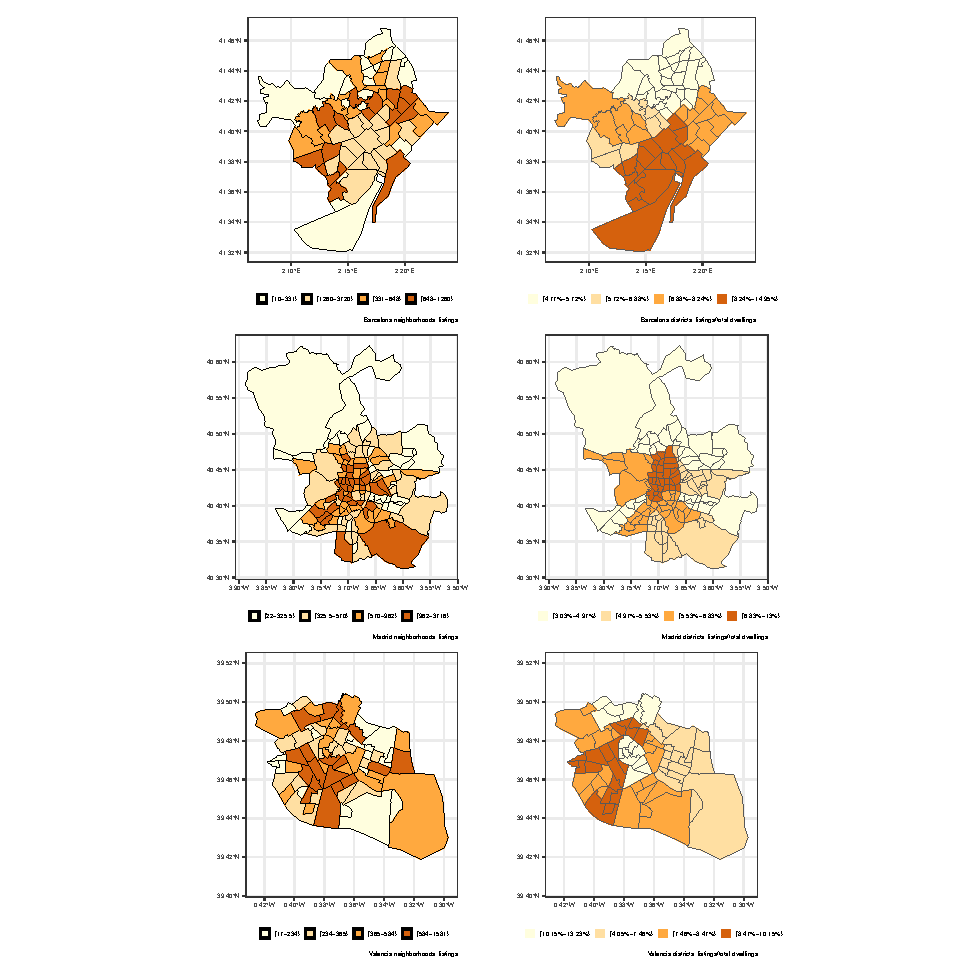
\includegraphics{main_EPB_files/figure-latex/figure-listings-1.pdf}
\caption{\label{fig:all-polygons}\DIFaddFL{Listings by neighborhood (left column)
and percentage of listings relative to total dwellings (right column).
Barcelona (Top), Madrid (Center), and Valencia (Bottom).}}
\end{figure}

\DIFaddend \hypertarget{points-of-interest}{%
\subsection{Points of Interest}\label{points-of-interest}}

The last \DIFdelbegin \DIFdel{block of data }\DIFdelend \DIFaddbegin \DIFadd{data object }\DIFaddend included in the \DIFdelbegin \DIFdel{data }\DIFdelend package is a set of Points of
Interest in each city as an object of the class list. The name of the
list includes the name of the city with the suffix '\_POIS'. These lists
include three elements: (i) the coordinates of the city center, the
central business district; (ii) a set of coordinates that define the
main street of each city; and (iii) the coordinates of the metro
stations.

\DIFdelbegin %DIFDELCMD < \hypertarget{anonymizing}{%
%DIFDELCMD < \section{Anonymizing the data set}\label{anonymizing}}
%DIFDELCMD < %%%
\DIFdelend \DIFaddbegin \hypertarget{anonymizing}{%
\section{Masking the prices}\label{anonymizing}}
\DIFaddend 

To comply with Spanish regulations, \DIFdelbegin \DIFdel{two }\DIFdelend \DIFaddbegin \DIFadd{three }\DIFaddend variables were slightly
modified to provide \DIFaddbegin \DIFadd{a measure of }\DIFaddend anonymity. A masking process was
applied to asking prices and location (coordinates).

In terms of the asking prices, the original values were obfuscated with
the addition or subtraction of a random percentage of their original
values, ranging from \DIFdelbegin \DIFdel{-2.5\% to +2.5\%}\DIFdelend \DIFaddbegin \DIFadd{\(-2.5%
\) to \(+2.5%
\)}\DIFaddend . Since asking prices are usually multiples of 1,000, after the first
price modification, the prices were aligned to multiples of 1,000.

\DIFdelbegin %DIFDELCMD < \begin{algorithm}[!ht]
%DIFDELCMD <  \KwData{all idealista listings}
%DIFDELCMD <  \KwResult{all idealista listings with masked coordinates}
%DIFDELCMD <  %%%
\DIFdel{initialization\;
 }%DIFDELCMD < \For{each listing L}{
%DIFDELCMD <   take geographical location of L as $(X,Y)$
%DIFDELCMD <   \Repeat{this stop condition}{
%DIFDELCMD <     take a random angle $\alpha$ from 0 to 360 degrees
%DIFDELCMD <     take a distance $R$ as a random value from 30 to 60 meters
%DIFDELCMD <     determine a new point $(X',Y')$ calculated as a point located $R$ with the angle $\alpha$
%DIFDELCMD <   }
%DIFDELCMD <   set $(X',Y')$ as the new location for the listing L
%DIFDELCMD <  }
%DIFDELCMD <  %%%
%DIFDELCMD < \caption{%
{%DIFAUXCMD
\DIFdel{Coordinate displacement process for anonymisation purposes}}
 %DIFAUXCMD
%DIFDELCMD < \label{algo:coordinates-displacement}
%DIFDELCMD < \end{algorithm}
%DIFDELCMD < %%%
\DIFdelend \DIFaddbegin \DIFadd{To understand the implications of this masking process, we use some
standard results from algebra of random variables. The masked prices
\(P\) are given by: }\[
\DIFadd{P = RP\cdot \epsilon
}\]
\DIFaddend 

\DIFaddbegin \noindent \DIFadd{where \(RP\) are the original (raw) prices, and \(\epsilon\)
is a random variable drawn from the uniform distribution with parameters
\(a=0.975\) and \(b=1.025\): }\[
\DIFadd{f(\epsilon) = 
\begin{cases}
\frac{1}{b - a} & \text{for } a\le \epsilon \le b\\
0 & \text{otherwise}
\end{cases}
}\]

\DIFadd{The expectation of \(\epsilon\) given these parameters is: }\[
\DIFadd{E}[\DIFadd{\epsilon}] \DIFadd{= \frac{a+b}{2} = \frac{0.975 + 1.025}{2} = 1
}\]

\noindent \DIFadd{and the variance of \(\epsilon\) is: }\[
\DIFadd{\mathrm{V}[\epsilon]=\frac{(b - a)^2}{12} = \frac{1}{4800}
}\]

\DIFadd{Therefore, the expectation of the masked prices is: }\[
\DIFadd{\mathrm{E}[P] = \mathrm{E}[RP\cdot \epsilon] = \mathrm{E}[RP]\cdot \mathrm{E}[\epsilon] = \mathrm{E}[RP]
}\]

\DIFadd{In other words, the masked prices \(P\) are an unbiased version of the
raw prices \(RP\).
}

\DIFadd{Considering that \(RP\) and \(\epsilon\) are independent, the variance
of the masked prices is as follows: }\[
\DIFadd{\mathrm{V}[P] = \mathrm{V}[RP\cdot \epsilon] = \mathrm{V}[RP]\cdot \mathrm{V}[\epsilon] + \mathrm{V}[RP]\cdot (\mathrm{E}[\epsilon])^2 + \mathrm{V}[\epsilon]\cdot(\mathrm{E}[RP])^2
}\]

\DIFadd{Since \(\mathrm{E}[\epsilon] = 1\), we have that: }\[
\DIFadd{\mathrm{V}[P] = \mathrm{V}[RP]\cdot \mathrm{V}[\epsilon] + \mathrm{V}[RP] + \mathrm{V}[\epsilon]\cdot(\mathrm{E}[RP])^2 = \mathrm{V}[RP]\cdot (1 + \mathrm{V}[\epsilon]) + \mathrm{V}[\epsilon]\cdot(\mathrm{E}[RP])^2
}\]

\DIFadd{Solving for \(\mathrm{V}[RP]\), and replacing the expectation of the raw
prices by its unbiased version (\(\mathrm{E}[P]\)), yields the variance
of the raw prices: }\[
\DIFadd{\mathrm{V}[RP] = \frac{\mathrm{V}[P] - \frac{1}{4800}\cdot (\mathrm{E}[P])^2}{1 + \frac{1}{4800}}
}\]

\DIFadd{Table \ref{tab:variance} reports the mean and the standard deviation
(i.e., the square root of the variance) of the prices in the package,
and the standard deviation (again, the square root of the variance) of
the raw prices calculated using the formula above. This is done for each
quarter and for the full year. The last column of the table can be read
as an inflation factor. We see that the variance of the masked prices is
inflated with respect to the variance of the original values by less
than \(1\%\) in all cases examined. Users can use the formula above to
calculate the inflation of the variance if they use subsamples other
than those shown, to assess the potential impacts of the masking (e.g.,
when computing intervals of confidence).
}

\begin{table}

\caption{\label{tab:variance-inflation-calculations}\label{tab:variance}\DIFaddFL{Inflation of the variance of masked prices with respect to raw prices}}
\centering
\fontsize{9}{11}\selectfont
\begin{threeparttable}
\begin{tabular}[t]{llllll}
\toprule
\DIFaddFL{City }& \DIFaddFL{Period }& \DIFaddFL{mean(P) }& \DIFaddFL{sd(P) }& \DIFaddFL{sd(RP) }& \DIFaddFL{sd(P)/sd(RP)}\\
\midrule
 & \DIFaddFL{Q1 }& \DIFaddFL{405,166.8 }& \DIFaddFL{308,623.8 }& \DIFaddFL{308,536.2 }& \DIFaddFL{1.00057}\\
\cmidrule{2-6}
 & \DIFaddFL{Q2 }& \DIFaddFL{388,053.5 }& \DIFaddFL{252,520.5 }& \DIFaddFL{252,432.1 }& \DIFaddFL{1.0007}\\
\cmidrule{2-6}
 & \DIFaddFL{Q3 }& \DIFaddFL{382,692.5 }& \DIFaddFL{268,880.9 }& \DIFaddFL{268,796.1 }& \DIFaddFL{1.00063}\\
\cmidrule{2-6}
 & \DIFaddFL{Q4 }& \DIFaddFL{398,157.8 }& \DIFaddFL{275,459.3 }& \DIFaddFL{275,370.6 }& \DIFaddFL{1.00064}\\
\cmidrule{2-6}
\multirow{-5}{*}{\raggedright\arraybackslash BARCELONA} & \DIFaddFL{2018 }& \DIFaddFL{395,770.6 }& \DIFaddFL{281,554.8 }& \DIFaddFL{281,467.5 }& \DIFaddFL{1.00062}\\
\cmidrule{1-6}
 & \DIFaddFL{Q1 }& \DIFaddFL{404,960.8 }& \DIFaddFL{447,935.3 }& \DIFaddFL{447,850.5 }& \DIFaddFL{1.00038}\\
\cmidrule{2-6}
 & \DIFaddFL{Q2 }& \DIFaddFL{367,527.5 }& \DIFaddFL{383,093.9 }& \DIFaddFL{383,017.2 }& \DIFaddFL{1.0004}\\
\cmidrule{2-6}
 & \DIFaddFL{Q3 }& \DIFaddFL{365,467.2 }& \DIFaddFL{359,118.3 }& \DIFaddFL{359,042.2 }& \DIFaddFL{1.00042}\\
\cmidrule{2-6}
 & \DIFaddFL{Q4 }& \DIFaddFL{410,952.7 }& \DIFaddFL{428,852.7 }& \DIFaddFL{428,767 }& \DIFaddFL{1.0004}\\
\cmidrule{2-6}
\multirow{-5}{*}{\raggedright\arraybackslash MADRID} & \DIFaddFL{2018 }& \DIFaddFL{396,110.1 }& \DIFaddFL{417,074.4 }& \DIFaddFL{416,991.8 }& \DIFaddFL{1.0004}\\
\cmidrule{1-6}
 & \DIFaddFL{Q1 }& \DIFaddFL{204,836.5 }& \DIFaddFL{187,957.4 }& \DIFaddFL{187,914.6 }& \DIFaddFL{1.00046}\\
\cmidrule{2-6}
 & \DIFaddFL{Q2 }& \DIFaddFL{176,661 }& \DIFaddFL{141,002.4 }& \DIFaddFL{140,964.6 }& \DIFaddFL{1.00054}\\
\cmidrule{2-6}
 & \DIFaddFL{Q3 }& \DIFaddFL{188,189.4 }& \DIFaddFL{167,146 }& \DIFaddFL{167,106.6 }& \DIFaddFL{1.00047}\\
\cmidrule{2-6}
 & \DIFaddFL{Q4 }& \DIFaddFL{208,523.5 }& \DIFaddFL{183,452.7 }& \DIFaddFL{183,409 }& \DIFaddFL{1.00048}\\
\cmidrule{2-6}
\multirow{-5}{*}{\raggedright\arraybackslash VALENCIA} & \DIFaddFL{2018 }& \DIFaddFL{199,678.3 }& \DIFaddFL{177,156 }& \DIFaddFL{177,114.1 }& \DIFaddFL{1.00047}\\
\bottomrule
\end{tabular}
\begin{tablenotes}
\item \textit{\DIFaddFL{Note: }} 
\item \DIFaddFL{P: masked prices; 
}\item \DIFaddFL{RP: raw prices; 
}\item \DIFaddFL{sd: standard deviation (square root of the variance)
}\end{tablenotes}
\end{threeparttable}
\end{table}

\DIFaddend With respect to the location of the dwelling, a spatial masking process
was implemented to maintain the spatial properties of the original data
set. The coordinates of each listing were displaced using a stochastic
procedure. The listings were recorded using coordinates contained in
maximum and minimum displacement circles, as shown in Figure
\ref{fig:Anonymizing} (left). To preserve inclusion in a neighborhood,
the spatial masking procedure was constrained to ensure that the masked
coordinates remained in the original neighborhood of the listing.

\DIFaddbegin \begin{algorithm}[!ht]
 \KwData{all idealista listings}
 \KwResult{all idealista listings with masked coordinates}
 \DIFadd{initialization\;
 }\For{each listing L}{
  take geographical location of L as $(X,Y)$
  \Repeat{this stop condition}{
    take a random angle $\alpha$ from 0 to 360 degrees
    take a distance $R$ as a random value from 30 to 60 meters
    determine a new point $(X',Y')$ calculated as a point located $R$ with the angle $\alpha$
  }
  set $(X',Y')$ as the new location for the listing L
 }
 \caption{\DIFadd{Coordinate displacement process for masking purposes}}
 \label{algo:coordinates-displacement}
\end{algorithm}

\DIFaddend Algorithm \ref{algo:coordinates-displacement} iteratively displaces the
coordinates of each listing with a minimum distance and a maximum
distance with the restriction that the new coordinates do not fall into
a different neighborhood. This ensures that neighborhood attributes are
preserved.

Figure \ref{fig:Anonymizing} (right) shows the histogram of the
displacements in meters for all the listings in the city of Valencia.
The average distance between the original and masked coordinates is 45
meters.

\begin{figure}

{\centering 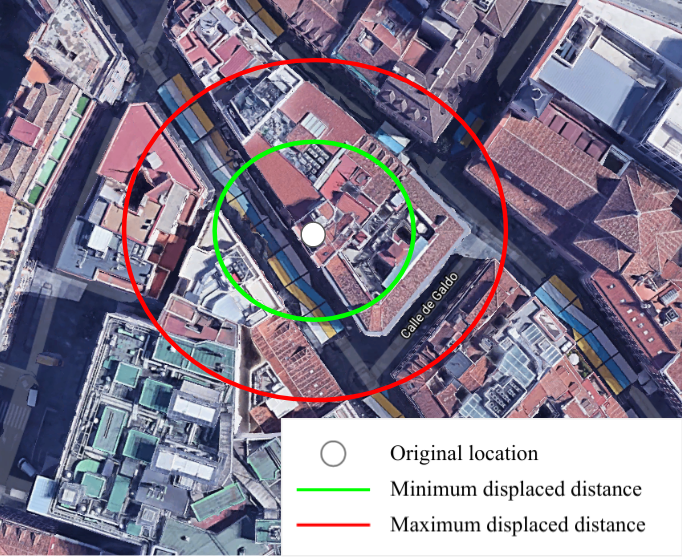
\includegraphics[width=0.29\linewidth,height=0.2\textheight]{EPB_files/points-moved-image} 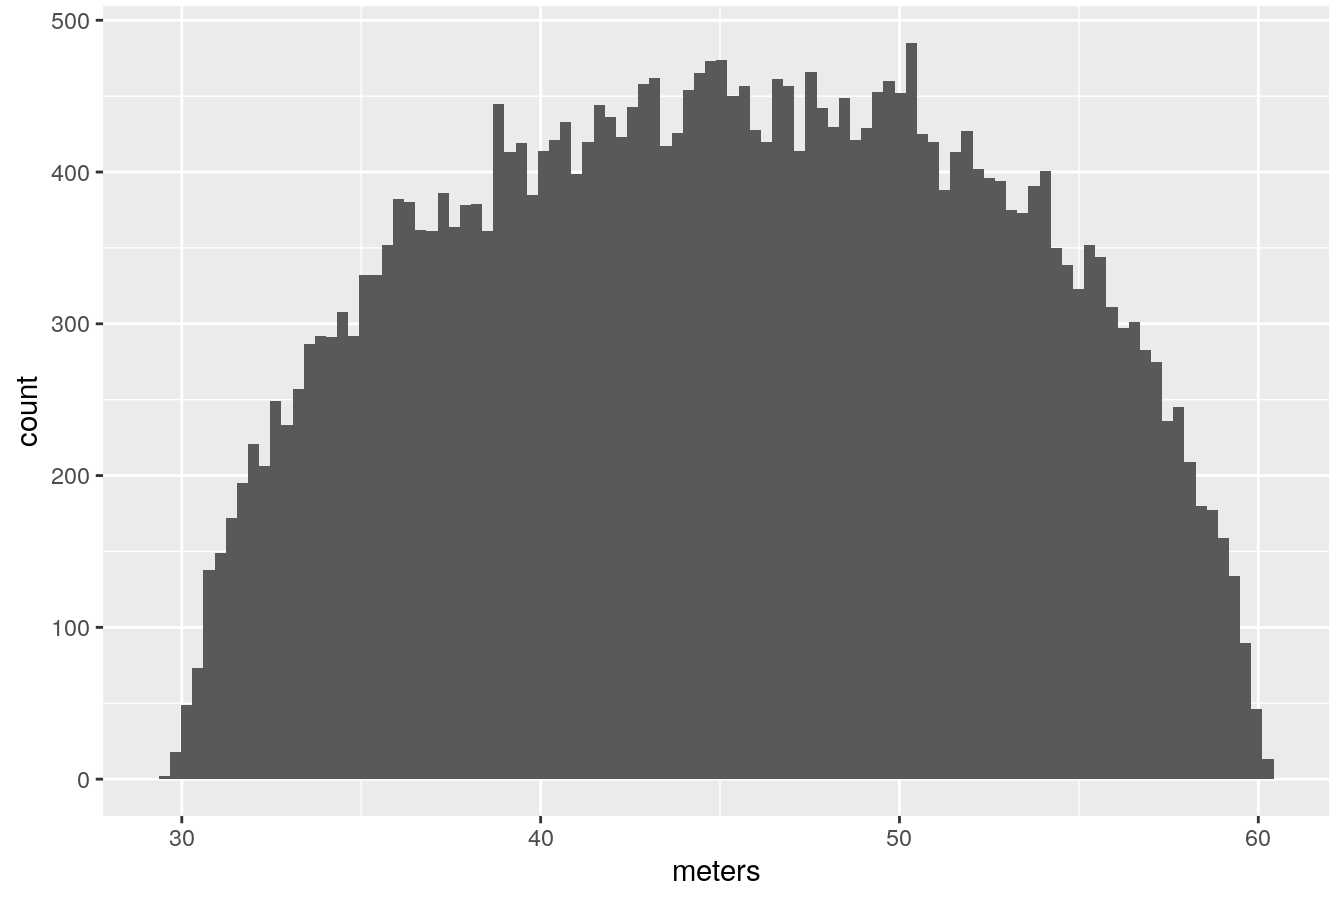
\includegraphics[width=0.37\linewidth,height=0.2\textheight]{EPB_files/coordinates-valencia} 

}

\caption{\label{fig:Anonymizing}(Left) Masking coordinates. Spatial range. (Right) Coordinate displacement in meters (Valencia)}\DIFdelbeginFL %DIFDELCMD < \label{fig:unnamed-chunk-2}
%DIFDELCMD < %%%
\DIFdelendFL \DIFaddbeginFL \label{fig:figure-masking-coordinates}
\DIFaddendFL \end{figure}

\hypertarget{conclusion}{%
\section{Conclusion}\label{conclusion}}

This paper describes a data product of a geo-referenced micro-data set
of Spain's three largest cities. This \DIFdelbegin \DIFdel{is an excellent data product to
help understand the complex mechanisms related to the }\DIFdelend \DIFaddbegin \DIFadd{data product can be of value to
support research into the mechanisms of }\DIFaddend housing market and housing
prices. Researchers can apply hedonic models with spatial effects,
\DIFdelbegin \DIFdel{identifying housing submarketsor }\DIFdelend \DIFaddbegin \DIFadd{identify housing submarkets, or experiment with }\DIFaddend machine learning
techniques. The data product can also be used for educational proposes
and teaching activities. \DIFaddbegin \DIFadd{To the best of our knowledge, this is the
largest, publicly available data set of its type that is also analysis
ready and fully documented.
}\DIFaddend 

\hypertarget{declaration-of-competing-interest}{%
\section{Declaration of Competing
Interest}\label{declaration-of-competing-interest}}

\DIFdelbegin \DIFdel{Author One and author }\DIFdelend \DIFaddbegin \DIFadd{Authors One and }\DIFaddend Two are employed by Idealista. They have been granted
permission to share the data presented in this article. None of the
authors have financial interests or personal relationships which have,
or could be perceived to have, influenced the work reported in this
article.

\hypertarget{acknowledgments}{%
\section{Acknowledgments}\label{acknowledgments}}

The authors wish to thank Alessandro Galesi for their support in the
paper revision and Juan Ramón Selva for collecting and cleaning the
spatial data. This work has been partially funded by the Spanish
Ministry of Economy and Competitiveness Grants PID2019-107800GB-100\DIFaddbegin \DIFadd{, but
it was not funded by any of Canada's research councils.
}\DIFaddend 

\bibliographystyle{sageh}
\bibliography{bibEPB.bib}


\end{document}
